\chapter{The in-medium similarity renormalization group}\label{ch:imsrg}

The in-medium similarity renormalization group
is a modern \abinitio{} many-body method
that extends the renormalization group approach of decoupling energy scales
to many-body calculations.
It is a non-perturbative wave function expansion method,
in the same vein as coupled cluster,
but it operates on the operators rather than the wave function.
It is remarkably flexible,
with favorable scaling with system size
and the ability to target many different observables,
and its invention and development has contributed strongly
to the rapid expansion of \abinitio{} theoretical calculations of medium-mass nuclei.
In this chapter, we introduce the IM-SRG formalism.
We then discuss the topics of truncation scheme, generator selection,
and approaches to solving the flow equations.

\section{Basic formalism}

As a reminder from Section~\ref{sec:srg},
the idea behind the SRG is
the construction of a continuous unitary transformation of the Hamiltonian
\begin{equation}
  H(s) = U(s) H U^{\dagger}(s)\,,
\end{equation}
which can be obtained by solving the flow equation
\begin{equation}\label{eq:srg_flow_equation_imsrg}
  \frac{d H(s)}{ds} = [\eta(s), H(s)]\,,
\end{equation}
with the anti-Hermitian generator $\eta(s)$.
The solution of this flow equation with vacuum normal-ordered operators,
the free-space SRG,
is appealing in that the evolved operators are not system specific
and can be generally used for many-body calculations of nuclei and nuclear matter.
However, the free-space SRG evolution can only be done consistently
in the two- and three-body spaces for nuclear systems,
leaving out induced higher-body operators.

The idea behind the IM-SRG is to solve Eq.~\ref{eq:srg_flow_equation_imsrg} in-medium,
that is, to normal order with respect to a reference state before solving the flow equations.
Starting from a Hamiltonian with a one-, two- and three-body part
\begin{equation}
  H = \onebodyop{H} + \twobodyop{H} + \threebodyop{H}\,,
\end{equation}
our normal-ordered Hamiltonian matrix elements are given by
\begin{align}
  E &\equiv \hnozero = \sum_i \onebodyop{H}_{ii} + \frac{1}{2}\sum_{ij} \twobodyop{H}_{ijij} + \frac{1}{6} \sum_{ijk} \threebodyop{H}_{ijkijk}\,, \\
  f_{pq} &\equiv \hnoone_{pq} = \onebodyop{H}_{pq} + \sum_i \twobodyop{H}_{piqi} + \frac{1}{2} \sum_{ij} \threebodyop{H}_{pijqij} \,, \\
  \Gamma_{pqrs} &\equiv \hnotwo_{pqrs} = \twobodyop{H}_{pqrs} + \sum_i \threebodyop{H}_{pqirsi} \,,  \\
  W_{pqrstu} &\equiv \hnothree_{pqrstu} = \threebodyop{H}_{pqrstu} \,,
\end{align}
where we have introduced the conventional names
for zero-, one-, two-, and three-body normal-ordered parts of the Hamiltonian,
$E$, $f$, $\Gamma$, and $W$,
used in the literature.
As a reminder,
indices $p$, $q$, $r$, \ldots\ run over all single-particle states,
indices $i$, $j$, $k$, \ldots\ run over holes,
single-particle states occupied in the reference state,
and indices $a$, $b$, $c$, \ldots\ run over particles,
single-particle states unoccupied in the reference state.

In general, the generator $\eta(s)$ has one- through $A$-body normal-ordered parts
\begin{equation}
  \eta(s) = \sum_{i=1}^A \eta^{(i)}(s)\,.
\end{equation}
For now, we leave $\eta(s)$ unspecified beyond its required anti-Hermiticity,
which causes it to not have a zero-body part.
We discuss the choice of generator in Section~\ref{sec:imsrg_generator}.
Concretely, our initial normal-ordered Hamiltonian is
\begin{equation}
  \begin{split}
    H = &\,E
  + \sum_{pq} f_{pq} \noref{\crea{p} \annih{q}} \\
    &+ \frac{1}{{(2!)}^2} \sum_{pqrs} \Gamma_{pqrs} \noref{\crea{p} \crea{q} \annih{s} \annih{r}}\\
    &+ \frac{1}{{(3!)}^2} \sum_{pqrstu} W_{pqrstu} \noref{\crea{p} \crea{q} \crea{r} \annih{u} \annih{t} \annih{s}}\,,
  \end{split}
\end{equation}
and our generator is
\begin{equation}
  \begin{split}
    \eta(s) = &
  \sum_{pq} \eta^{(1)}_{pq}(s) \noref{\crea{p} \annih{q}} \\
    &+ \frac{1}{{(2!)}^2} \sum_{pqrs} \eta^{(2)}_{pqrs}(s) \noref{\crea{p} \crea{q} \annih{s} \annih{r}}\\
    &+ \frac{1}{{(3!)}^2} \sum_{pqrstu} \eta^{(3)}_{pqrstu}(s) \noref{\crea{p} \crea{q} \crea{r} \annih{u} \annih{t} \annih{s}}\\
    &+ \ldots \,.
  \end{split}
\end{equation}

The evaluation of the right-hand side of Eq.~\ref{eq:srg_flow_equation_imsrg} then reduces to
the evaluation of commutators of normal-ordered products,
\begin{equation}
  \left[\noref{\crea{p_1} \ldots \crea{p_M} \annih{q_M} \ldots \annih{q_1}},
  \noref{\crea{r_1} \ldots \crea{r_N} \annih{s_N} \ldots \annih{s_1}}\right]\,,
\end{equation}
which can be simplified into a sum of normal-ordered operators
using the generalized Wick's theorem (see Eq.~\ref{eq:gen_wicks_theorem}).
The commutator of an $M$-body operator $A^{(M)}$ and an $N$-body operator $B^{(N)}$
will in general have contributions of $|M-N|$-body operators through $M+N-1$-body operators,
\begin{equation}
  [A^{(M)}, B^{(N)}] = \sum_{k=|M-N|}^{M+N-1}C^{(k)}\,.
\end{equation}

The right-hand side can then be broken up into zero- through $A$-body parts.
We then identify the zero-body part of the right-hand side with $dE/ds$,
the one-body part with $df_{pq}/ds$, and so on.
This makes it obvious that
even if the initial Hamiltonian and generator contain only up to three-body operators
the IM-SRG evolution induces higher-body operators,
all the way up to $A$-body operators after a couple integration steps,
resulting in coupled flow equations for the zero- through $A$-body parts
of the Hamiltonian.
Note that one must also ensure the antisymmetry of the right-hand sides of the two-,
three-, and higher-body flow equations
so the matrix elements remain antisymmetric.

The discussion here has been focused on the Hamiltonian,
but the IM-SRG can also be used to evolve other operators,
\begin{equation}
  \frac{dO}{ds} = \comm{\eta(s)}{O(s)}\,,
\end{equation}
where $O$ has also been normal ordered with respect to our reference state $\refgnd$.
Since the generator $\eta(s)$ should be the same for the evolution of $H$ and $O$
and the reconstruction of the unitary transformation from the evolved form of $H$
is not possible,
$H$ and $O$ must naively be evolved simultaneously.
In Section~\ref{sec:imsrg_magnus}, we discuss an alternative approach to solving the IM-SRG flow equations
that allows for the construction of the unitary transformation,
resulting in easy evolution of other operators along with the Hamiltonian.

\section{Truncation schemes}

As is the case with the free-space SRG,
it is not feasible to do the full $A$-body evolution,
and the flow equations must be truncated at some $B$-body level.
However, the situation is not quite the same as with the free-space SRG.\@
Because the initial normal ordering shifts information about higher-body operators
into lower-body normal-ordered operators
and the continuous normal ordering absorbs information about induced higher-body operators
into lower-body normal-ordered operators,
the truncated IM-SRG flow equations still approximately evolve higher-body operators
(in the free-space sense)
using only the reduced $B$-body flow equations.
In the following sections,
we discuss truncating the IM-SRG at the two-body and three-body level,
yielding the so-called IM-SRG(2) and IM-SRG(3) truncations respectively.

\subsection{IM-SRG(2)}

Truncating the flow equation at the two-body level amounts to assuming
\begin{align}
  H(s) &\approx E(s) + f(s) + \Gamma(s)\,,\\
  \eta(s) &\approx \eta^{(1)}(s) + \eta^{(2)}(s)\,.
\end{align}
In this approximation,
we are not including the three-body part of the initial Hamiltonian exactly.
However, the three-body force \textit{does} contribute
as it was used in obtaining the normal-ordered zero-, one-, and two-body parts
of the Hamiltonian.
This is known as the normal-ordered two-body (NO2B) approximation,
which has been quite successful in nuclear many-body applications.

Using the generalized Wick's theorem,
which yields the fundamental commutators in Appendix A of Ref.~\cite{Herg15imsrgphysrep},
one arrives at the flow equations for the Hamiltonian
\begin{align}
  \phantom{\frac{d\Gamma_{pqrs}}{ds}}
  &\begin{aligned}
    \mathllap{\frac{dE}{ds}} &= \sum_{pq} n_{p} \bar{n}_{q}
    (\genone_{pq} f_{qp} - f_{pq} \genone_{qp})\\
    &\quad + \frac{1}{4} \sum_{pqrs} n_{p}n_{q}\bar{n}_r \bar{n}_s
    (\gentwo_{pqrs} \Gamma_{rspq} - \Gamma_{pqrs}\gentwo_{rspq})\,,
  \end{aligned}\label{eq:imsrg2_0body}\\
  &\begin{aligned}
    \mathllap{\frac{df_{pq}}{ds}} &=
    \sum_{r}(\genone_{pr} f_{rq} - f_{pr} \genone_{rq}) \\
    &\quad+\sum_{rs}(n_r - n_s)(\genone_{rs}\Gamma_{sprq} - f_{rs}\gentwo_{sprq}) \\
    &\quad+\frac{1}{2}\sum_{rst}(\bar{n}_r \bar{n}_s n_t + n_r n_s \bar{n}_t)
    (\gentwo_{tprs} \Gamma_{rstq} - \Gamma_{tprs} \gentwo_{rstq})\,,
  \end{aligned}\\
  &\begin{aligned}
    \mathllap{\frac{d\Gamma_{pqrs}}{ds}} &=
    \sum_{t}(1 - P_{pq})(\genone_{pt}\Gamma_{tqrs} - f_{pt}\gentwo_{tqrs}) \\
    &\quad - \sum_{t}(1 - P_{rs})(\genone_{tr}\Gamma_{pqts} - f_{tr}\gentwo_{pqts}) \\
    &\quad + \frac{1}{2}\sum_{tu}(1 - n_{t} - n_{u})(\gentwo_{pqtu}\Gamma_{turs} - \Gamma_{pqtu}\gentwo_{turs}) \\
    &\quad + \sum_{tu} (n_t - n_u)(1 - P_{pq})(1 - P_{rs})\gentwo_{tpur}\Gamma_{uqts}\,,
  \end{aligned}\label{eq:imsrg2_2body}
\end{align}
where $n_p$ are the occupation numbers of the reference state,
$\bar{n}_p = 1 - n_p$,
the $s$-dependence has been suppressed,
and the permutation operator $P_{pq}$ exchanges the indices $p$ and $q$
in the following expression.

Eqs.~\ref{eq:imsrg2_0body}-\ref{eq:imsrg2_2body} are solved by integrating
from $s=0$ towards $s\rightarrow\infty$ with the initial conditions
$E(0) = E$, $f(0) = f$, and $\Gamma(0)=\Gamma$.
Given appropriate decoupling (see Section~\ref{sec:imsrg_generator}),
$E(\infty)$ gives the energy of the state targeted by the reference state,
for our applications typically the ground state.
The cost of this integration is dominated by the final two terms in Eq.~\ref{eq:imsrg2_2body},
which scale like $\mathcal{O}(N^6)$,
where $N$ is the size of the single-particle basis for the calculation.
Another nice property is that the flow equation,
due to being a commutator many-body expansion,
generates only connected diagrams and thus ensures size extensivity~\cite{Herg15imsrgphysrep}.
This is true for any $B$-body truncation.

\subsection{IM-SRG(3)}

Truncating at the three-body level allows one to exactly include initial three-body forces.
One assumes
\begin{align}
  H(s) &\approx E(s) + f(s) + \Gamma(s) + W(s)\,,\\
  \eta(s) &\approx \genone(s) + \gentwo(s) + \genthree(s)\,,
\end{align}
yielding additional terms with commutators of $\genthree$ and $W$
with zero- through two-body operators
and a commutator between $\genthree$ and $W$.
The flow equations are
\begin{align}
  \phantom{\frac{dW_{pqrstu}}{ds}}
  &\begin{aligned}
    \mathllap{\frac{dE}{ds}} &= \sum_{pq} n_{p} \bar{n}_{q}
    (\genone_{pq} f_{qp} - f_{pq} \genone_{qp})\\
    &\quad + \frac{1}{4} \sum_{pqrs} n_{p}n_{q}\bar{n}_r \bar{n}_s
    (\gentwo_{pqrs} \Gamma_{rspq} - \Gamma_{pqrs}\gentwo_{rspq})\\
    &\quad + \frac{1}{36}\sum_{pqrstu} n_p n_q n_r \bar{n}_s \bar{n}_t \bar{n}_u
    (\genthree_{pqrstu} W_{stupqr} - W_{pqrstu} \genthree_{stupqr})\,,
  \end{aligned}\label{eq:imsrg3_0body}\\
  &\begin{aligned}
    \mathllap{\frac{df_{pq}}{ds}} &=
    \sum_{r}(\genone_{pr} f_{rq} - f_{pr} \genone_{rq}) \\
    &\quad+\sum_{rs}(n_r - n_s)(\genone_{rs}\Gamma_{sprq} - f_{rs}\gentwo_{sprq}) \\
    &\quad+\frac{1}{2}\sum_{rst}(\bar{n}_r \bar{n}_s n_t + n_r n_s \bar{n}_t)
    (\gentwo_{tprs} \Gamma_{rstq} - \Gamma_{tprs} \gentwo_{rstq}) \\
    &\quad - \frac{1}{4} \sum_{rstu}(n_r n_s \bar{n}_t \bar{n}_u -\bar{n}_r \bar{n}_s n_t n_u)
    (\gentwo_{turs} W_{rspqtu} - \Gamma_{turs} \genthree_{rspqtu}) \\
    &\quad + \frac{1}{12}\sum_{rstuv}
             (n_r n_s \bar{n}_t \bar{n}_u \bar{n}_v + \bar{n}_r \bar{n}_s n_t n_u n_v)
             (\genthree_{rsptuv} W_{tuvrsq} - W_{rsptuv} \genthree_{tuvrsq})\,,
  \end{aligned}\\
  &\begin{aligned}
    \mathllap{\frac{d\Gamma_{pqrs}}{ds}} &=
    \sum_{t}(1 - P_{pq})(\genone_{pt}\Gamma_{tqrs} - f_{pt}\gentwo_{tqrs}) \\
    &\quad - \sum_{t}(1 - P_{rs})(\genone_{tr}\Gamma_{pqts} - f_{tr}\gentwo_{pqts}) \\
    &\quad + \frac{1}{2}\sum_{tu}(1 - n_{t} - n_{u})(\gentwo_{pqtu}\Gamma_{turs} - \Gamma_{pqtu}\gentwo_{turs}) \\
    &\quad + \sum_{tu} (n_t - n_u)(1 - P_{pq})(1 - P_{rs})\gentwo_{tpur}\Gamma_{uqts} \\
    &\quad + \sum_{tu} (n_t - n_u)(\genone_{tu} W_{upqtrs} - f_{tu} \genthree_{upqtrs})\\
    &\quad - \frac{1}{2} \sum_{tuv} (n_t \bar{n}_u \bar{n}_v + \bar{n}_t n_u n_v)
              (1 - P_{rs})(\gentwo_{uvtr} W_{tpquvs} - \Gamma_{uvtr} \genthree_{tpquvs}) \\
    &\quad + \frac{1}{2} \sum_{tuv} (n_t \bar{n}_u \bar{n}_v + \bar{n}_t n_u n_v)
              (1 - P_{pq})(\gentwo_{uvtp} W_{trsuvq} - \Gamma_{uvtp} \genthree_{trsuvq}) \\
    &\quad + \frac{1}{6} \sum_{tuvw}(n_t \bar{n}_u \bar{n}_v \bar{n}_w -\bar{n}_t n_u n_v n_w)
              (\genthree_{tpquvw} W_{uvwtrs} - W_{tpquvw} \genthree_{uvwtrs}) \\
    &\quad + \frac{1}{4} \sum_{tuvw}(\bar{n}_t \bar{n}_u n_v n_w -n_t n_u \bar{n}_v \bar{n}_w)
              (1 - P_{pq})(1 - P_{rs}) \genthree_{tupvws} W_{vwqtur}\,,
  \end{aligned}\label{eq:imsrg3_2body} \\
  &\begin{aligned}
    \mathllap{\frac{dW_{pqrstu}}{ds}} &=
    \sum_{v} P(p/qr) (\genone_{pv} W_{vqrstu} - f_{pv} \genthree_{vqrstu}) \\
    &\quad - \sum_{v} P(s/tu) (\genone_{vs} W_{pqrvtu} - f_{vs} \genthree_{pqrvtu}) \\
    &\quad + \sum_{v} P(pq/r) P(s/tu)
              (\gentwo_{pqsv} \Gamma_{vrtu} - \Gamma_{pqsv} \gentwo_{vrtu}) \\
    &\quad + \frac{1}{2} \sum_{vw} (1 - n_v - n_w) P(pq/r)
              (\gentwo_{pqvw} W_{vwrstu} - \Gamma_{pqvw} \genthree_{vwrstu}) \\
    &\quad - \frac{1}{2} \sum_{vw} (1 - n_v - n_w) P(s/tu)
              (\gentwo_{vwtu} W_{pqrsvw} - \Gamma_{vwtu} \genthree_{pqrsvw}) \\
    &\quad + \frac{1}{6} \sum_{vwx} (n_v n_w n_x + \bar{n}_v \bar{n}_w \bar{n}_x)
              (\genthree_{pqrvwx} W_{vwxstu} - W_{pqrvwx} \genthree_{vwxstu}) \\
    &\quad + \frac{1}{2} \sum_{vwx} (n_v n_w \bar{n}_x + \bar{n}_v \bar{n}_w n_x)
              P(pq/r)P(s/tu)\\
    &\qquad \qquad \times (\genthree_{vwrxtu} W_{xpqvws} -\genthree_{xqrvwu} W_{pvwstx})\,,
  \end{aligned}\label{eq:imsrg3_3body}
\end{align}
Here, $P(pq/r) = 1 - P_{pr} - P_{qr}$ and $P(p/qr) = 1 - P_{pq} - P_{pr}$
ensure the antisymmetry of the three-body indices.

It is clear that the final two terms in Eq.~\ref{eq:imsrg3_3body}
dominate the cost of the integration,
scaling like $\mathcal{O}(N^9)$ in the size of our single-particle basis.
In the absence of an initial three-body operator,
the third term in Eq.~\ref{eq:imsrg3_3body},
the three-body part of the commutator of two two-body operators,
induces a three-body operator,
which leads to the contribution of all other terms later in the integration.

We would also like to note that
in the derivation of the flow equations here
the only assumption that was made was that
two- and three-body matrix elements are appropriately antisymmetric.
In particular, unlike several other references in the literature,
for instance Refs.~\cite{Herg15imsrgphysrep,Tsuk10imsrg},
the flow equations here do not assume $f$, $\Gamma$ and $W$ are Hermitian
(which of course they are).
While this assumption allows for the simplification of certain terms
(nothing that changes the scaling of the terms however),
it limits the expressions to only commutators of anti-Hermitian and Hermitian operators.
In Section~\ref{sec:imsrg_magnus},
we require the commutator of two anti-Hermitian operators,
for which the right-hand sides of
Eqs.~\ref{eq:imsrg2_0body}-\ref{eq:imsrg2_2body}
and Eqs.~\ref{eq:imsrg3_0body}-\ref{eq:imsrg3_3body}
are equally valid.
For numerical implementations,
it is a good idea to implement each of the fundamental commutators separately,
to allow for validation and fine-grained optimization in the most expensive commutators.

\section{Generator selection}\label{sec:imsrg_generator}

\begin{figure}[t]
\setlength{\unitlength}{0.8\columnwidth}
  \begin{center}
  \begin{picture}(1.0000,0.5500)
   \put(0.0350,0.0450){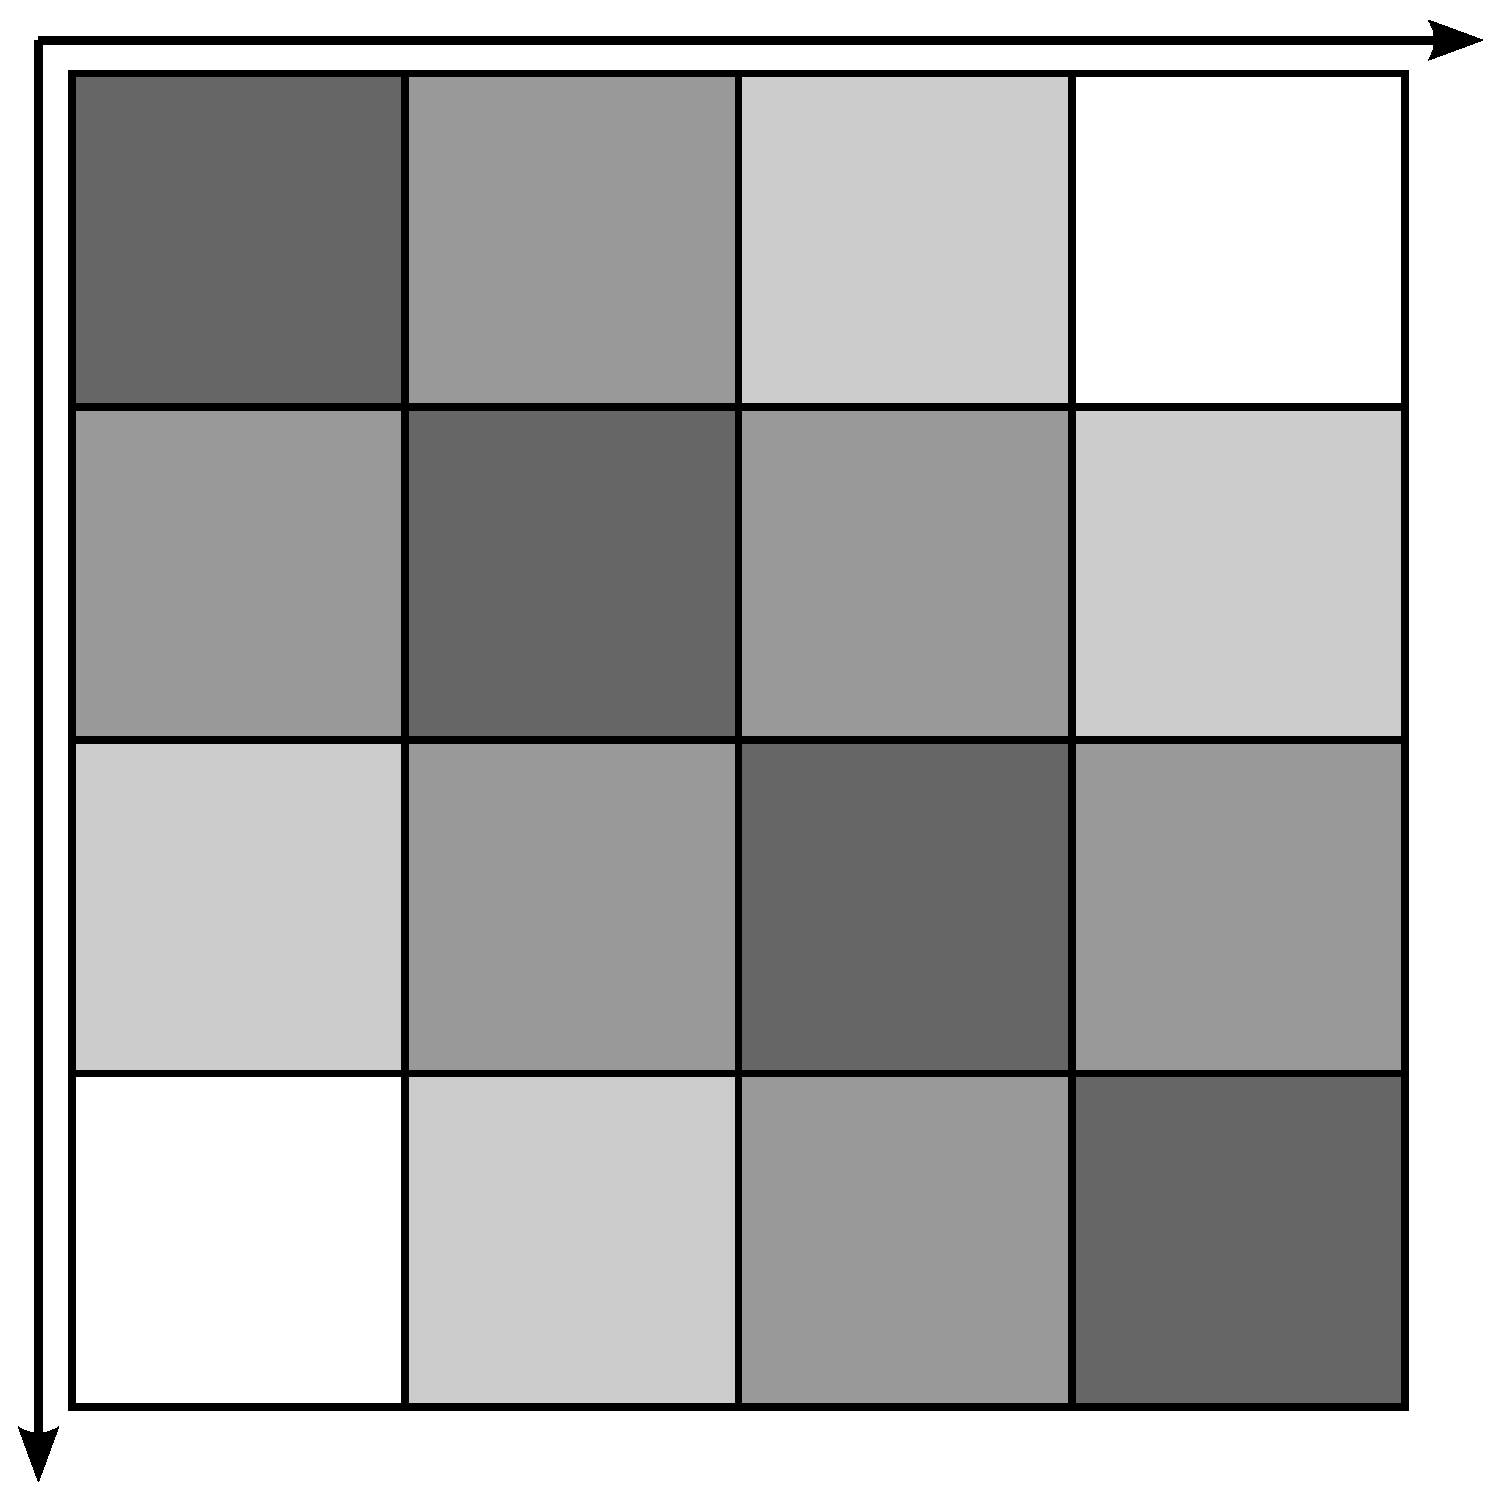
\includegraphics[width=0.46\unitlength]{proposal/doc/images/external/H_initial.eps}}
   \put(0.5400,0.0450){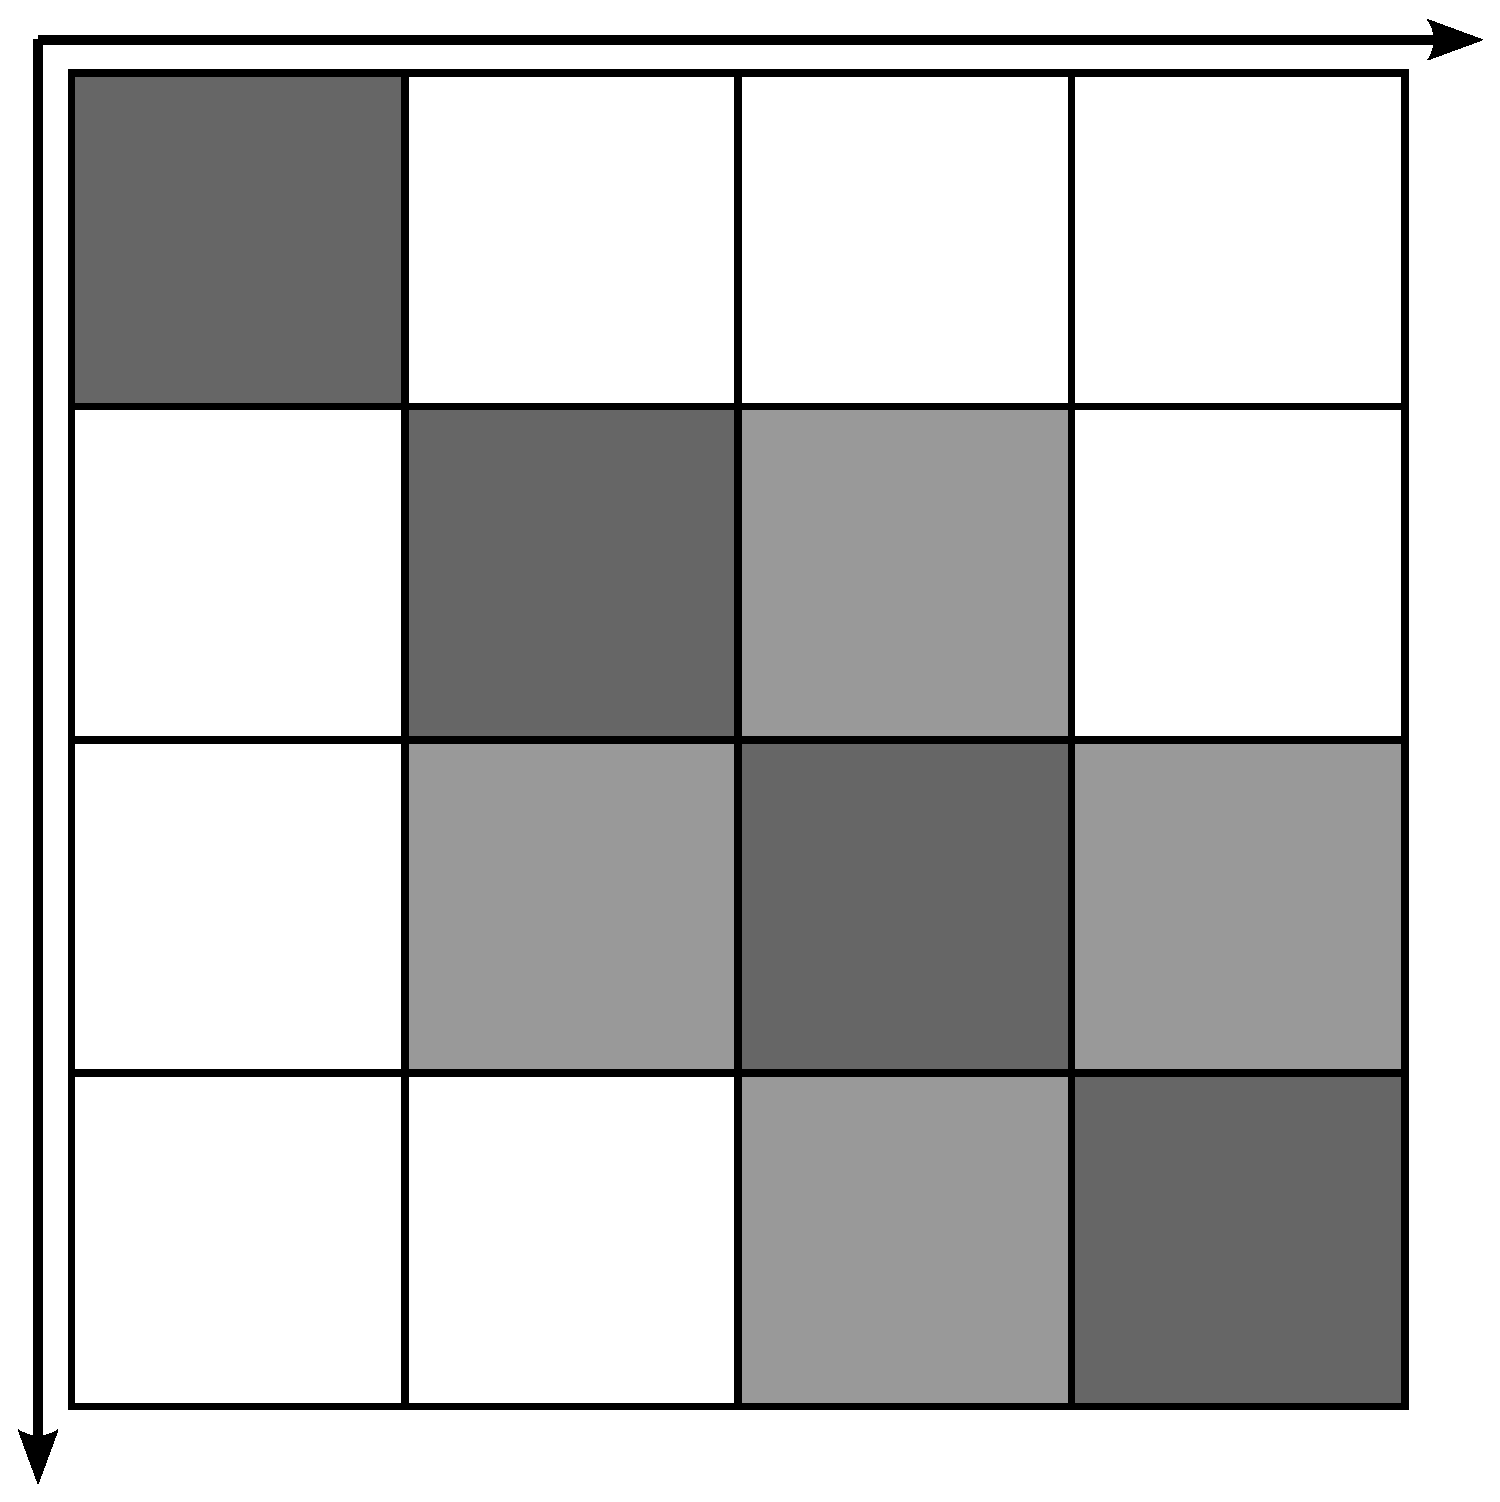
\includegraphics[width=0.46\unitlength]{proposal/doc/images/external/H_IMSRG_3ph_decoupling.eps}}
   \put(0.0100,0.0000){\parbox{0.5\unitlength}{\centering$\braket{i|H(0)|j}$}}
   \put(0.5200,0.0000){\parbox{0.5\unitlength}{\centering$\braket{i|H(\infty)|j}$}}

   \put(0.0500,0.5100){\parbox{0.11\unitlength}{\centering\footnotesize0p0h}}
   \put(0.1600,0.5100){\parbox{0.11\unitlength}{\centering\footnotesize1p1h}}
   \put(0.2630,0.5100){\parbox{0.11\unitlength}{\centering\footnotesize2p2h}}
   \put(0.3650,0.5100){\parbox{0.11\unitlength}{\centering\footnotesize3p3h}}
   \put(0.5500,0.5100){\parbox{0.11\unitlength}{\centering\footnotesize0p0h}}
   \put(0.6600,0.5100){\parbox{0.11\unitlength}{\centering\footnotesize1p1h}}
   \put(0.7630,0.5100){\parbox{0.11\unitlength}{\centering\footnotesize2p2h}}
   \put(0.8650,0.5100){\parbox{0.11\unitlength}{\centering\footnotesize3p3h}}
  %
   \put(0.0100,0.4320){\parbox{0.11\unitlength}{\rotatebox{90}{\centering\footnotesize0p0h}}}
   \put(0.0100,0.3235){\parbox{0.11\unitlength}{\rotatebox{90}{\centering\footnotesize1p1h}}}
   \put(0.0100,0.2175){\parbox{0.11\unitlength}{\rotatebox{90}{\centering\footnotesize2p2h}}}
   \put(0.0100,0.1100){\parbox{0.11\unitlength}{\rotatebox{90}{\centering\footnotesize3p3h}}}

   \put(0.5100,0.4320){\parbox{0.11\unitlength}{\rotatebox{90}{\centering\footnotesize0p0h}}}
   \put(0.5100,0.3235){\parbox{0.11\unitlength}{\rotatebox{90}{\centering\footnotesize1p1h}}}
   \put(0.5100,0.2175){\parbox{0.11\unitlength}{\rotatebox{90}{\centering\footnotesize2p2h}}}
   \put(0.5100,0.1100){\parbox{0.11\unitlength}{\rotatebox{90}{\centering\footnotesize3p3h}}}
  \end{picture}
  \end{center}
  \caption[
    Schematic diagram
    showing the minimal decoupling scheme
    taken in the IM-SRG.\@
  ]{\label{fig:imsrg_decoupling}
    Schematic diagram
    showing the minimal decoupling scheme
    taken in the IM-SRG.\@
    Figure taken from Ref.~\cite{Herg15imsrgphysrep}.
  }
\end{figure}

So far, we have not discussed specific choices of our generator $\eta$.
The possible definitions of $\eta$ hinge on the specification
of our so-called ``off-diagonal'' Hamiltonian $H_{od}$,
the part of the Hamiltonian we wish to suppress
to ensure appropriate decoupling in the remaining ``diagonal'' part.
In Section~\ref{sec:srg},
we saw that the generator choice
$\eta = \comm{T_{\text{rel}}}{H(s)}$
leads to the decoupling of any two states
with a decay scale set by the difference in their kinetic energy expectation values.
The result is that the Hamiltonian evolves towards a diagonal form,
providing vastly improved convergence
and allowing many-body calculations to use significantly smaller modelspaces.

To identify the desired decoupling for the IM-SRG,
we begin by considering the Hamiltonian in the basis spanned by
our reference state $\refgnd$ and
$n$-particle $n$-hole ($npnh$) excitations of the reference state,
\begin{equation}
  \{\refgnd, \refhp{i}{a}, \refhp{ij}{ab}, \refhp{ijk}{abc}, \ldots \}\,.
\end{equation}
For a Hamiltonian with only one- and two-body operators,
as is the approximation after normal-ordering for the IM-SRG(2) truncation,
the Hamiltonian in this basis is schematically represented
in the left panel of Fig.~\ref{fig:imsrg_decoupling}.
It is band-diagonal and only able to couple an $npnh$ excitation
to $(n\pm2)p(n\pm2)h$ excitations.
For a Hamiltonian with a three-body part,
the band diagonal grows to include $(n\pm3)p(n\pm3)h$ excitations.

For the IM-SRG,
a decoupling towards a true diagonal form is no longer a good idea,
as one must avoid inducing significant three-body terms in the IM-SRG(2)
or four- and higher-body terms in the IM-SRG(3)
to maintain the validity of the truncation.
The alternative is a minimal decoupling scheme,
where the sole objective is to decouple the reference state $\refgnd$
from all $npnh$ excitations,
as shown in the right panel of Fig.~\ref{fig:imsrg_decoupling}.
Achieving this decoupling gives us the energy of the state $E$
in the zero-body part of the normal-ordered Hamiltonian
and the corresponding eigenstate by applying the unitary transformation
to the reference state, $U^{\dagger}(\infty)\refgnd$.
For some finite truncation of the flow equations,
this result is of course only approximate.

Now that we know we want to suppress the matrix elements
which couple $\refgnd$ to its excitations,
we want to identify which parts of our normal-ordered Hamiltonian
these matrix elements correspond to.
For the couplings between $\refgnd$ and $1p1h$ excitations, we find
\begin{align}
  \phantom{\braket{\Phi | H |\Phi_{i}^{a}}}
  &\begin{aligned}
    \mathllap{\braket{\Phi | H |\Phi_{i}^{a}}} &= \braket{\Phi | H \noref{\crea{a} \annih{i}}| \Phi}
  \end{aligned}\\
  &\begin{aligned}
    \mathllap{}&= E \braket{\Phi | \noref{\crea{a} \annih{i}} | \Phi} \\
    &\quad + \sum_{pq} f_{pq} \braket{\Phi |\noref{\crea{p}\annih{q}} \noref{\crea{a} \annih{i}} | \Phi} \\
    &\quad + \sum_{pqrs} \Gamma_{pqrs}
    \braket{\Phi |\noref{\crea{p} \crea{q} \annih{s} \annih{r}}\noref{\crea{a} \annih{i}} | \Phi}
  \end{aligned}\\
  &\begin{aligned}
    \mathllap{}&= \sum_{pq} f_{pq} \delta_{pi} \delta_{qa} n_{i} \bar{n}_{a}
  \end{aligned}\\
  &\begin{aligned}
    \mathllap{}&= f_{ia}\,.
  \end{aligned}
\end{align}
Via similar calculations, one finds
\begin{samepage}
  \begin{subequations}
    \begin{align}
      \begin{split}
        \braket{\Phi_{i}^{a} | H | \Phi} &= f_{ai}\,,
      \end{split}\\
      \begin{split}
        \braket{\Phi | H | \Phi_{ij}^{ab}} &= \Gamma_{ijab}\,,
      \end{split}\\
      \begin{split}
        \braket{\Phi_{ij}^{ab} | H | \Phi} &= \Gamma_{abij}\,,
      \end{split}\\
      \begin{split}
        \braket{\Phi | H | \Phi_{ijk}^{abc}} &= W_{ijkabc}\,,
      \end{split}\\
      \begin{split}
        \braket{\Phi_{ijk}^{abc} | H | \Phi} &= W_{abcijk}\,.
      \end{split}
    \end{align}
  \end{subequations}
\end{samepage}
We define our ``off-diagonal'' normal-ordered Hamiltonian then to be
\begin{equation}
  \begin{split}
    H_{od} \equiv & \sum_{ia}\left(f_{ia} \noref{\crea{i}\annih{a}}
                                + f_{ai} \noref{\crea{a}\annih{i}}\right) \\
                  & + \frac{1}{{(2!)}^2}\sum_{ijab} \left(
                      \Gamma_{ijab} \noref{\crea{i}\crea{j}\annih{b}\annih{a}}
                      + \Gamma_{abij} \noref{\crea{a}\crea{b}\annih{j}\annih{i}}
                    \right) \\
                  & + \frac{1}{{(3!)}^2}\sum_{ijkabc} \left(
                      W_{ijkabc} \noref{\crea{i}\crea{j}\crea{k}\annih{c}\annih{b}\annih{a}}
                      + W_{abcijk} \noref{\crea{a}\crea{b}\crea{c}\annih{k}\annih{j}\annih{i}}
                    \right)\,.
  \end{split}
\end{equation}
We are now in a position where we can define generators that suppress these matrix elements
over the course of the flow.

Wegner's original ansatz for the generator of the SRG flow equation is
\begin{equation}
  \eta(s) = \comm{H_d(s)}{H_{od}(s)}\,,
\end{equation}
where $H_d = H - H_{od}$~\cite{Wegn94srg}.
When using $H_{od}$ as defined above,
one can evaluate the commutator truncating at the two- or three-body level
depending on the truncation scheme,
giving the one-, two-, and three-body components of $\eta$
in the same form as Eqs.~\ref{eq:imsrg3_0body}-\ref{eq:imsrg3_3body}.
A perturbative analysis of the flow equations with this choice of generator,
as is done in Ref.~\cite{Herg16imsrglecnotes},
reveals that the two-body ``off-diagonal'' matrix elements are suppressed like
\begin{equation}
  \Gamma_{abij}(s) \approx \Gamma_{abij}(0) \exp(-{(\Delta_{abij})}^{2} s)\,,
\end{equation}
where $\Delta_{abij}$ are the energy denominators.
There are multiple options for these energy denominators,
corresponding to different partitionings in MBPT (see Section~\ref{sec:mbpt}).
We choose to focus on the M{\o}ller-Plesset denominators,
with $\Delta_{abij} = \epsilon_{abij}$ from Eq.~\ref{eq:mp_energy_denom}.
Another alternative is the Epstein-Nesbet denominators
(see Ref.~\cite{Shav09mbpt_cc_book} for details).

We have included the Wegner generator in this discussion for completeness
but will not use it in any applications.
One reason for this is that the Wegner generator is simply more expensive to construct
than the alternatives,
which give explicit expressions for the matrix elements of $\eta$,
resulting in scaling of $\mathcal{O}(N^4)$ and $\mathcal{O}(N^6)$ for IM-SRG(2) and IM-SRG(3),
respectively.
This is to be contrasted with the evaluation of a full commutator,
which scales like $\mathcal{O}(N^6)$ and $\mathcal{O}(N^9)$ for IM-SRG(2) and IM-SRG(3).
Additionally, the Wegner generator causes the system of differential equations
to be much more stiff,
making the integration much more expensive
(in terms of storage and computational requirements)
than for other generators.

The following generators directly construct the matrix elements of $\eta$, working with a basic form of
\begin{equation}
  \begin{split}
    \eta \equiv & \sum_{ia}\left(\genone_{ia} \noref{\crea{i}\annih{a}}
                                + \genone_{ai} \noref{\crea{a}\annih{i}}\right) \\
                  & + \frac{1}{{(2!)}^2} \sum_{ijab} \left(
                      \gentwo_{ijab} \noref{\crea{i}\crea{j}\annih{b}\annih{a}}
                      + \gentwo_{abij} \noref{\crea{a}\crea{b}\annih{j}\annih{i}}
                    \right) \\
                  & + \frac{1}{{(3!)}^2} \sum_{ijkabc} \left(
                      \genthree_{ijkabc} \noref{\crea{i}\crea{j}\crea{k}\annih{c}\annih{b}\annih{a}}
                      + \genthree_{abcijk} \noref{\crea{a}\crea{b}\crea{c}\annih{k}\annih{j}\annih{i}}
                    \right)\,,
  \end{split}
\end{equation}
where we note that for $\eta$ to be anti-Hermitian, the matrix elements must fulfill
\begin{subequations}
  \begin{align}
    \begin{split}
      \genone_{ia} &= - \genone_{ai}\,,
    \end{split} \\
    \begin{split}
      \gentwo_{ijab} &= - \gentwo_{abij}\,,
    \end{split} \\
    \begin{split}
      \genthree_{ijkabc} &= - \genthree_{abcijk}\,.
    \end{split}
  \end{align}
\end{subequations}
The White generator corresponds to the choice
\begin{align}
  \genone_{ia}(s) &= \frac{f_{ia}(s)}{\Delta_{ia}(s)}\,,\\
  \gentwo_{ijab}(s) &= \frac{\Gamma_{ijab}(s)}{\Delta_{ijab}(s)}\,,\\
  \genthree_{ijkabc}(s) &= \frac{W_{ijkabc}(s)}{\Delta_{ijkabc}(s)}\,,
\end{align}
where the antisymmetry of the denominators automatically gives the desired anti-Hermiticity~\cite{Whit02generator}.
The White generator suppresses off-diagonal matrix elements like
\begin{equation}
  \Gamma_{abij}(s) \approx \Gamma_{abij}(0) \exp(-s)\,,
\end{equation}
that is, it suppresses all off-diagonal matrix elements with the same decay scale,
regardless of the energy differences between the states.
This is unusual and not strictly speaking in line with the renormalization group approach,
where large energy-difference modes are integrated out first.
However, we are interested in $H(\infty)$ and $E(\infty)$,
and in this limit all generators that suppress $H_{od}$ produce identical results
for $E(\infty)$ and $U^{\dagger}(\infty)\refgnd$,
up to truncation effects.

A potential difficulty with the White generator arises
when one of the energy denominators becomes very small,
leading to large matrix elements of $\eta$
and thus extremely large derivatives in the right-hand side of the flow equation.
This can be mitigated by a variation of the standard White generator,
the arctan generator,
with generator matrix elements defined as
\begin{align}
  \genone_{ia}(s) &= \frac{1}{2}\text{arctan}\left(\frac{2f_{ia}(s)}{\Delta_{ia}(s)}\right)\,,\\
  \gentwo_{ijab}(s) &= \frac{1}{2}\text{arctan}\left(\frac{2\Gamma_{ijab}(s)}{\Delta_{ijab}(s)}\right)\,,\\
  \genthree_{ijkabc}(s) &= \frac{1}{2}\text{arctan}\left(\frac{2W_{ijkabc}(s)}{\Delta_{ijkabc}(s)}\right)\,,
\end{align}
where the arctan function regularizes any possible large matrix elements arising due to small energy denominators.

The final generator we discuss here is the imaginary-time generator,
which was ostensibly inspired by imaginary-time evolution techniques
in Quantum Monte Carlo methods~\cite{Herg15imsrgphysrep}.
Its matrix elements are defined as
\begin{align}
  \genone_{ia}(s) &= \text{sign}(\Delta_{ia}(s))f_{ia}(s)\,, \\
  \gentwo_{ijab}(s) &= \text{sign}(\Delta_{ijab}(s))\Gamma_{ijab}(s)\,, \\
  \genthree_{ijkabc}(s) &= \text{sign}(\Delta_{ijkabc}(s))W_{ijkabc}(s)\,.
\end{align}
A perturbative analysis of the flow equations with this generator choice shows
that off-diagonal matrix elements are suppressed like
\begin{equation}
  \Gamma_{abij}(s) \approx \Gamma_{abij}(0) \exp(-|\Delta_{abij}|s)\,.
\end{equation}
The sign function in the definition of the generator ensures that
there is an absolute value around the energy denominator in the exponential,
giving a suppression for all matrix elements instead of an enhancement for some.
We also note here that the imaginary-time generator produces a ``proper'' RG flow,
where matrix elements coupling large energy differences are suppressed
before those coupling smaller energy differences.

\section{The Magnus expansion}\label{sec:imsrg_magnus}

Working with Eqs.~\ref{eq:imsrg2_0body}-\ref{eq:imsrg2_2body}
and~\ref{eq:imsrg3_0body}-\ref{eq:imsrg3_3body},
one can solve the IM-SRG by numerically integrating
the system of ordinary differential equations (ODEs)
to obtain the energy and the expectation values of other observables in the targeted state.
This approach has two main challenges:
First, the flow equations need to be solved to high precision,
as otherwise numerical effects destroy the unitarity of the transformation
even in the absence of any truncation.
This necessitates the application of sophisticated ODE solvers
to minimize this numerical error.
These solvers require the allocation of several times the memory requirement
of two- and three-body operators,
which is already quite a lot (on the order of GB or tens of GB),
and the evaluation of each integration step is substantially more expensive
(providing the benefit of reduced accumulated numerical error)
than an Euler method.
This is incidentally also a reason the White, arctan, and imaginary-time generators
are preferred over the Wegner generator,
as the stiffness of the flow equations with the Wegner generator
requires the use of stiff ODE solvers,
which are even more expensive in terms of storage and computational cost
than their non-stiff counterparts.

Second, the evolution of other operators along with the Hamiltonian
requires them to be evolved in parallel in this approach.
This means that for every additional operator the memory and computational cost
increases by the amount that it would cost to just solve the Hamiltonian.
Furthermore, additional operators may increase the stiffness of the system of ODEs
as the integration scales for their matrix elements may differ from the Hamiltonian.
This challenge can be alleviated by the ability to construct the unitary transformation
for the evolution, $U(s)$.

This is the goal of the Magnus expansion approach to solving the IM-SRG flow equations~\cite{Morr15magnus}.
Given our definition of $\eta(s)$ following Eq.~\ref{eq:srg_flow_eq},
we get a differential equation for $U(s)$,
\begin{equation}
  \frac{dU(s)}{ds} = - \eta(s) U(s)\,,
\end{equation}
where $U(0) = 1$.
The formal integral of this differential equation is
\begin{equation}
  U(s) = \mathcal{T}_s\left[\exp(-\int_{0}^{s} ds' \eta(s'))\right]\,,
\end{equation}
where $\mathcal{T}_s$ is the time-ordering operator with respect to $s$~\cite{Dyso49timeorder}.

The Magnus expansion postulates that a solution of the form
\begin{equation}
  U(s) = \exp(\Omega(s))
\end{equation}
exists, where $\Omega(s)$ is anti-Hermitian and $\Omega(0) = 0$~\cite{Magn54magnus}.
To obtain $\Omega(s)$, one solves the differential equation of its expansion in $\eta(s)$,
\begin{equation}\label{eq:magnus_expansion}
  \frac{d \Omega(s)}{ds} = \sum_{k=0}^{\infty} \frac{B_{k}}{k!} ad^{k}_{\Omega(s)}(\eta(s))\,,
\end{equation}
where $B_{k}$ are the Bernoulli numbers
and $ad^{k}_{\Omega}$ are the recursively defined commutators,
\begin{align}
  ad^{0}_{\Omega(s)}(\eta(s)) &= \eta(s)\,, \\
  ad^{k}_{\Omega(s)}(\eta(s)) &= \comm{\Omega(s)}{ad^{k-1}_{\Omega(s)}(\eta(s))}\,.
\end{align}
The interested reader may refer to Ref.~\cite{Blan09magnusreview} for detailed review
of the Magnus expansion.

Here we note that $ad^{k}_{\Omega(s)}(\eta(s))$ is anti-Hermitian for all $k$,
thus truncating Eq.~\ref{eq:magnus_expansion} at any order
gives an exactly anti-Hermitian approximation to $d\Omega(s)/ds$,
which when integrated gives an exactly anti-Hermitian approximation to $\Omega(s)$.
Thus $U(s) = \exp(\Omega(s))$ is always exactly unitary,
regardless of accumulated numerical error in the solution for $\Omega(s)$.
This alleviates the requirement of using high-order ODE solvers to avoid numerical error,
and the solution of the IM-SRG flow equations in this approach
can proceed using a cheap numerical integrator,
for example a simple Euler method.

To apply the obtained unitary transformation to our Hamiltonian or some other operator,
we use the Baker-Campbell-Hausdorff (BCH) formula,
\begin{equation}\label{eq:bch_formula}
  H(s) = e^{\Omega(s)} H(0) e^{-\Omega(s)} = \sum_{k=0}^{\infty} \frac{1}{k!} ad^{k}_{\Omega(s)}(H(0))\,.
\end{equation}

To be concrete, the evaluation of the IM-SRG flow equations in the Magnus formalism
proceeds as follows:
\begin{enumerate}
  \item the generator $\eta(s)$ is constructed from $H(s)$,
  \item the derivative $d\Omega(s)/ds$ is obtained via Eq.~\ref{eq:magnus_expansion}
    and applied via a simple Euler method, % ($\Omega(s+ds) = \Omega(s) + ds d\Omega(s)/ds$),
  \item the new evolved Hamiltonian $H(s+ds)$ is obtained via Eq.~\ref{eq:bch_formula},
    %(alternatively, $H(s+ds)=\exp(ds d\Omega(s)/ds) H(s)\exp(-ds d\Omega(s)/ds)$),
\end{enumerate}
repeating these steps until $E$ is sufficiently converged.
For practical calculations, a few truncations must be made.
First, $H(s)$, $\eta(s)$, $\Omega(s)$, and all commutators must be truncated
at the $B$-body level,
leading to the Magnus(2) and Magnus(3) analogues to the IM-SRG(2) and IM-SRG(3) truncations.
Additionally, the Magnus and BCH expansions
(Eqs.~\ref{eq:magnus_expansion} and~\ref{eq:bch_formula})
must be truncated at some finite $k$.
For the Magnus expansion, we truncate the series when the norm of the $k$-th term
drops below a threshold $\epsilon_{\text{deriv}}$,
\begin{equation}
  \left\vert \frac{B_k || ad^{k}_{\Omega(s)}(\eta(s))||}{k!||\Omega(s)||} \right\vert < \epsilon_{\text{deriv}}\,.
\end{equation}
A similar condition can also be used for the truncation of the BCH expansion,
with the threshold $\epsilon_{\text{BCH}}$,
\begin{equation}
  \left\vert \frac{|| ad^{k}_{\Omega(s)}(H(0))||}{k!||\Omega(s)||} \right\vert < \epsilon_{\text{BCH}}\,.
\end{equation}
An alternative, for when one is only interested in the zero-body part of the evolving Hamiltonian,
is
\begin{equation}
  \left\vert \frac{\zerobodyop{ad^{k}_{\Omega(s)}(H(0))}}{k!} \right\vert < \epsilon_{\text{BCH}}\,.
\end{equation}

The Magnus expansion makes very clear the similarities and differences between
the IM-SRG and coupled cluster.
Both use a nested commutator expansion,
ensuring the connected nature of the expansion
and guaranteeing size extensivity.
The IM-SRG and CC seek to generate a similarity transformation
that decouples the reference state expectation value from the rest of the Hamiltonian.
However, in coupled cluster the cluster operator $T$ is non-Hermitian,
meaning that the BCH expansion for the similarity transformation truncates at a finite order.
The IM-SRG generates a unitary transformation,
which means $\Omega$, the Magnus analogue of the cluster operator,
is anti-Hermitian.
This leads to an infinite BCH expansion that must be truncated at some order.

In the next chapter, we present various results
for many-body calculations obtained using the IM-SRG.\@
Nearly all of these are done using the Magnus formalism,
as its computational benefits are invaluable to doing calculations
with three-body operators.

